% siminos/blog/BudCvi14edits.tex
% $Author: predrag $ $Date: 2016-04-08 14:53:32 -0400 (Fri, 08 Apr 2016) $
% Predrag created Nov 15 2013
% Predrag  switched to github.com                           Jul  8 2013
%           continues siminos/blog/dailyBlog.tex as of that date

\section{BudCvi14 PRL submission edits}

This section contains referee notes and
material which has not been included in
\emph{Reduction of the SO(2) symmetry for spatially extended dynamical
systems}\rf{BudCvi14}, {\tt siminos/slice/} in this repository,  and/or
Budanur Ph.D. thesis.
Please clean up whatever seems extraneous.

\begin{description}

\item[2014-03-09 Burak] Whether the fast turns close to $x_1 = 0$  in
    the reduced \KS\ solutions has a physical significance or not, is
    an open question.

High resolution in these regions of the reduced flow is an artifact of
slicing, however, this resolution could be used to gather qualitative
information of the flow by a \PoincSec.

Continuous symmetry reduction is the first step in construction of
symbolic dynamics of the \rpo s. We indeed took next steps and produced a
Poincar\'e return map, for the \twomode\ system that we used in this
paper to demonstrate symmetry reduction. A step-by-step introduction to
this will be our next publication.


\item[2014-04-02 Burak] Removed the following part:

\refRef{FrCv11} describes the instantaneous
jump in the reconstruction phase $\theta$ by $\pi$, induced by passage
through a general {\sliceBord}. As no numerical simulations of a
long-time ergodic trajectories known to us have ever actually encountered
this passage, the {\chartBord} point $\sspRed^*$ was engineered by hand
an initial condition to illustrate the jump in the phase.

\item[2014-04-15 Predrag] Removed this:
Any other \template\ that fixes the phase of the first Fourier mode would do just
as well.
\\{\bf Ruslan 2013-03-17} Is this right? If we fix the phase of the $n$-th
    mode, we will not have 'once and only once' cut, but $n$ cuts for the
    same value of the $n$-th mode phase.  In order to have a unique cut
    using modes with $n > 1$, we need to combine phases of several
    modes.
%    \BB{2013-04-01} {Changed ``any'' to ``first'' following Ruslan's comment. }

\item[2013-03-17 Ruslan] In \rf{SCD07} 16 FMs included the zero-mode, so that
the state space was 30-dimensional.  This is mainly because with
the total of $2^5$ values, the FFT is most efficient.

\item[2014-04-15 Ruslan]
Regarding  reffig {fig:f-ksconf}:
(b) Because this RPO has a shift of close to 11, it
looks almost periodic after two repetitions.  So, it is not immediately
clear that the reduced representation makes it exactly periodic (unless
we point this out).  Maybe use some other RPO, which is obviously not
periodic in full space, yet becomes obviously periodic in the reduced
space.

\item[2014-03-17 Ruslan]
Strictly speaking, since we are talking about numerical
    simulation of trajectories, the likelyhood is small, but {\em not} zero.
    Because numerical solutions are calculated within the finite-precision
    arithmetic, the '0' in the expression $\ssp_1 =0$ should be understood as
    {\em machine zero}, not zero on the real line.  The interval of real
    numbers identified with the machine zero has non-zero length.  At the
    same time, I don't see this as a problem from the computational point of
    view. (I remember reading something along these lines in a discussion
    between you and Evangelos in the blog.) So, maybe rather than saying that
    it can 'never' happen, we say that if it happens we know how to deal with
    it?

\item[Ruslan 2014-04-15] If I were a critical referee, I would comment that the
    'probabilistic' argument is rather weak and actually unnecessary.
    The problem of integrating near the slice border is introduced
    artificially by attempting to integrate equations on the slice.  Any
    trajectory that passes through zero of the 1-st Fourier mode will get
    stuck (i.e. take infinite time) in the time-rescaled formulation.
    There is no such problem in the full space: the orbit on the slice
    bounces off zero in the 1st mode, while $\theta$ is incremented by
    $\pi$ (or $-\pi$).

\item[2014-04-01 Burak]
Changed ``phase-fixing mode'' to ``first mode'' following
previous discussion on the ``unique'' intersection.


\item[2014-04-30 Evangelos] We say single intersection in next sentence, and every
group orbit is not true, so I removed: This \slice\ is global, as it
intersects every group orbit once and only once.

We define $a$ as real vector and we do not define $a_1$
as complex number, so I changed $a_1$ to $x_1$ in few places.


\item[2014-04-30 Evangelos] Removed mention of global symmetry reduction
from abstract and replaced it with a mention of global structures in state
space. The reason is that the abstract describes a direct product structure
(`state' and `phase' variables), while mathematicians (and many physicists)
know that the relevant global structure is a principal fibre bundle.
Most fibre bundles are not `trivial' (there is no global section, \ie, no global slice)
and therefore such a direct product structure can be given to the fibre bundle
only locally (Kevin Mitchell gave me hell about this as soon as I mentioned the
word `globally').

However, what we care about are global solutions or manifolds or attractors.
These are not global in the same sense as ``global symmetry reduction''
(and this is why the method slices locally but reduces globally).

\item[2014-05-09 Evangelos] By ``spatially extended systems'' we mean systems
with a spatial extent, usually described by PDEs (right?). However, for many
people, spatially extended is a system with size large
compared to the typical length scale of coherent structures. I hope reviewers
will not complain about this.

\item[2014-05-09 Evangelos] It would be actually interesting to think about slicing in
spatially extended systems of this narrower definition. In such systems periodicity is
not imposed by the box, but by the coherent structures themselves. This is why
higher mode or other physically motivated slices are important.

\item[2014-05-20 Evangelos] I went again through \refref{rowley_reduction_2003}, and I do
not understand why we credit them for time-rescaling transformation. Their transformation
is introduced to handle self-similar dynamics, and is associated with a fancy generalization
of equivariance. In the example of KS equation (which they study), this transformation does not
apply (simply because the system is equivariant in the usual sense) and they do not use it.
You have probably read this paper more carefully, so please
correct me if I am wrong. In any case, they do not seem to be concerned with slice border
singularities. Are you sure you want to cite them for this?

\item[2014-05-21 Burak]
I didn't understand Rowley's paper. It's probably different, but it is a
time rescaling that's why I thought we should cite them for doing it.

They state the equivariance as follows:
\[
v(g\cdot x) = \frac{1}{m(g)} g v(x)
\]
and call $m(g)$ a ``homomorphism''. Then rescale the time as:
\[
dt = m(g) d\tau .
\]
I think they address a subtlety and  generalize the method in some sense,
because we simply say that $v(g . x) = g v(x)$ when we state the
equivariance.

They probably still have the singularity in their phase velocity since in
their reduced velocity function (eq. 13) original velocity $(X(r))$ is not
multiplied by any factor, so may be we should not mention them at all.

\item[2014-05-21 Predrag] While we are used to travelling waves,
for which one can go to $\sspRed=\ssp-c \zeit$, they are thinking of
self-similar solutions, such as a diffusing wave, for which
$\sspRed=\ssp/\zeit^\alpha$ is the appropriate change of coordinates.
That looks very nice for the Burgers equation, their (45). They rescale
the spatial coordinate and arrive at the symmetry-reduced equation (46).
Here $u$ somehow turned into $r$, and $t$ into $\tau$, but I'm quite sure
this has nothing to do with our in-slice time.

Dropped the reference.

%\item[2014-08-25 Predrag]
%Replaced the abstract by Ruslan's version. Please edit as you see fit.
%Here is the old text:
%
%`Symmetry
%reduction' is a coordinate transformation which separates the state space
%into a lower-dimensional, symmetry-reduced state space, where every set
%of symmetry-equivalent states is represented by a single state, and
%`phase' coordinates which enable one to reconstruct the original, full
%state space dynamics. In the method of slices this reduction is achieved
%locally by cutting all group orbits  by a `slice'. Here we describe the
%`first Fourier mode slice', a simple application of the method to
%reduction of SO(2) symmetry, in which singularities in phase velocity
%close to the slice border are regularized by a time-scaling
%transformation. We show that global structures, such as chaotic
%attractors and unstable manifolds of traveling waves, are uncovered in
%the symmetry-reduced state space. We illustrate the method by applying it
%to a two-Fourier modes normal-form model and to the Kuramoto-Sivashinsky
%system.


\item[2014-08-15 Evangelos]
If you would like I could go through the first round of edits
implementing referee C suggestions, including removing the \twomode\
example.

\item[2014-08-24 Predrag]
No need to be timid - you are a coauthor, go ahead and edit, we can
always revert if there is something other coauthors do not like. Also, do
keep writing \refref{SCD09b}, you are the lead author on that one.

Removing \twomode\ example feels like throwing the baby out with the
water, hold off on that one for now.

\item[2014-09-03 Evangelos] Removed the 2-modes example from slice paper.
Introduced KSe earlier in the text in order to have a concrete example
of the passage from translations to SO(2) rotations, and from PDEs to ODEs.
Not done with this yet.

\paragraph{`\twoMode\ system'}
is a two-Fourier modes system studied in
\refref{Dang86,JoPro87,golubII,PoKno05}
as normal form
close to bifurcations off an $\SOn{2}$ invariant
\eqv. Our \twomode\ ODEs are\rf{BuBoCvSi14}:
\bea
\dot{x}_1 &=& (\mu_1    - r^2)\,x_1 + c_1\,(x_1 x_2 + y_1 y_2)
\,,\quad
 r^2 = x_1^2 + y_1^2\continue
\dot{y}_1 &=& (\mu_1    - r^2)\,y_1 + c_1\,(x_1 y_2 - x_2 y_1)
\continue
\dot{x}_2 &=& x_2 +  y_2 + x_1^2 - y_1^2  + a_2 x_2 r^2
\continue
\dot{y}_2 &=& -  x_2 + y_2 + 2\,x_1 y_1  + a_2 y_2 r^2
\,,
\label{twomode}
\eea
with parameter values $\mu_1 = -2.8,\, a_2 = -2.66,\,
c_1 = -7.75$ empirically chosen so the system exhibits chaos.
The flow satisfies the $\SOn{2}$ equivariance condition \refeq{eqvarcond}
by construction, with the Lie group element %\refeq{mmodeLieE2}
truncated
at the second mode. Furthermore, $r=0$ is a flow-invariant subspace.
That guarantees that in-slice
trajectories can only approach the \sliceBord\ $\hat{x}_1 =  0$, but never
cross it; hence the symmetry-reduced dynamics is confined to the \slice\
half-hyperplane for all times.

\refFig{f:twomode}\,(a) shows  the only \reqv\ of the \twomode\
system, a typical chaotic orbit, and its shortest \rpo\  projected down to 3
dimensions from the 4D \statesp. In the full \statesp\ the group
orbit of a \rpo\ is a torus, traced out ergodically by repeats of the
\rpo.
\refFig{f:twomode}\,(b) illustrates why symmetry-reduction is
absolute prerequisite to any analysis of the topology of a strange attractor.
Here, the same flow is shown in the three-dimensional symmetry-reduced
\slicePlane.
The full \statesp\ \reqv\ is reduced to an
\eqv\ and the \rpo\ to a \po. Once the drifts along the symmetry direction
have been quotiented out, a chaotic attractor, shaped by
the \reqv\ and the \eqv\ at the origin, is revealed\rf{BuBoCvSi14}.

%%%%%%%%%%%%%%%%%%%%%%%%%%%%%%%%%%%%%%%%%%%%%%%%%%%%%%%%%%%%%%%%%%%%%%%
\begin{figure}[tbp]
\centering
        \ifboyscout
(a)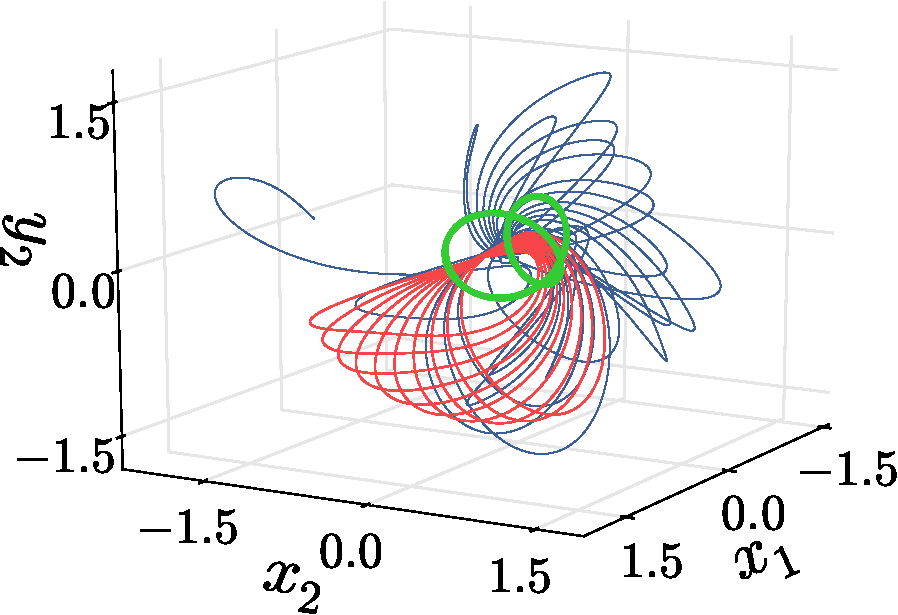
\includegraphics[width=0.41\textwidth]{BudCvi-2mode1}%
(b)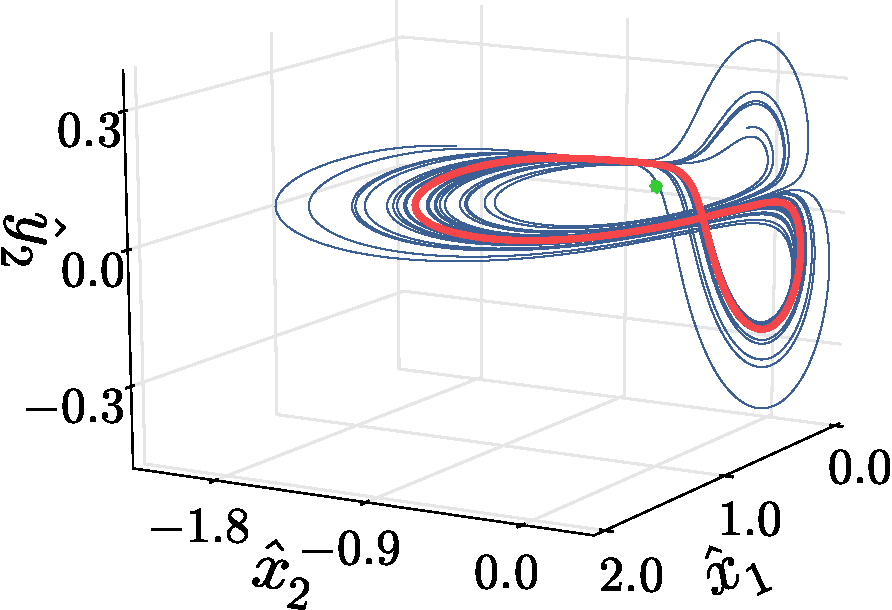
\includegraphics[width=0.41\textwidth]{BudCvi-2mode2}%
       \else
(a)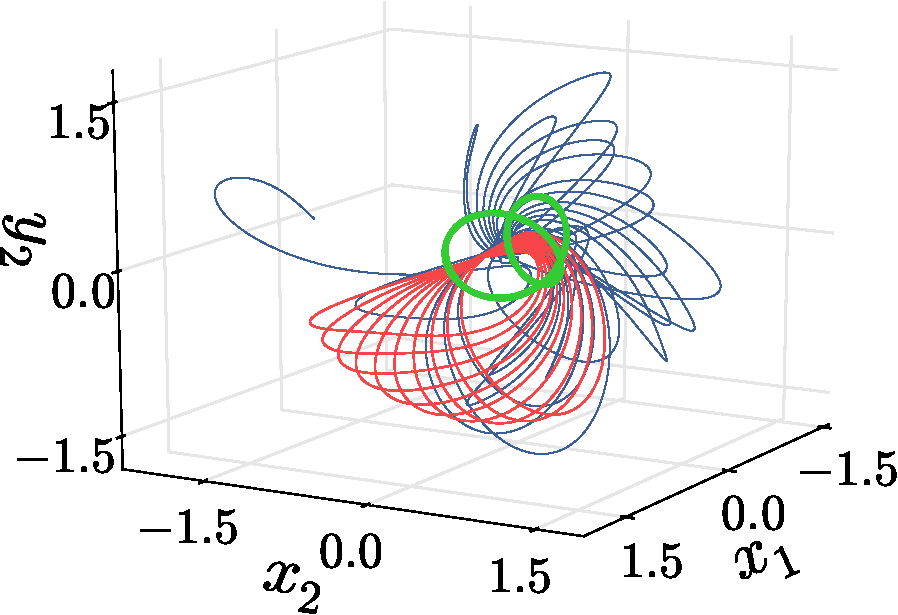
\includegraphics[width=0.21\textwidth]{BudCvi-2mode1}%
(b)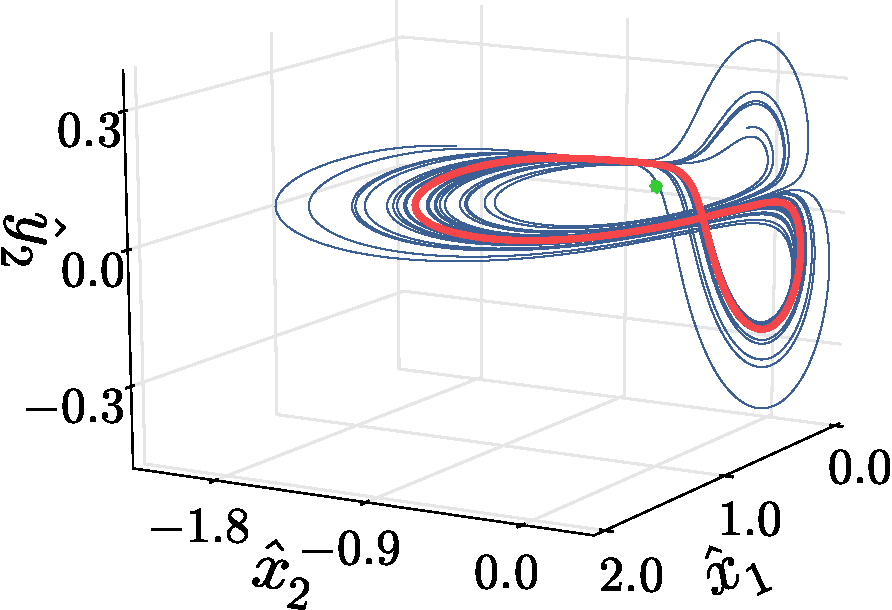
\includegraphics[width=0.21\textwidth]{BudCvi-2mode2}%
       \fi
\caption[]{
(Color online) The \twomode\ system:
A typical chaotic trajectory (blue), a trajectory spiraling out
from the \reqv\ (green), 10 repeats of the shortest
$\period{p} = 3.6415120$ \rpo\
(red) plotted in (a) a 3D projection of its
four-dimensional \statesp; (b) the three-dimensional \slicePlane.
}
\label{f:twomode}
\end{figure}
%%%%%%%%%%%%%%%%%%%%%%%%%%%%%%%%%%%%%%%%%%%%%%%%%%%%%%%%%%%%%%%%%%%%%%

\item[2014-09-12 Evangelos] Hugues offered to read and critique our slice manuscript (todays edition).
I have added his comments in the body of the text and I will try to edit the manuscript
to address them, as well as the referees comments this week. Please complain if you do not
see daily progress!

\item[2014-09-12 Evangelos] Hugues impression is that the article is not suitable for publication
in PRL at its present form. He considers it unnecessarirly hard, mathematical reading, while at the
end we do something very simple (fixing the phase of first Fourier mode).
He really thinks that a PRL should be readable by any physicist.
He also thinks that the example we present (KSe) is trivial. He is not convinced that this will work for NSe, and
says that we should have tried to publish only one PRL using both KSe and NSe as examples, so that it would
have maximum impact. He thinks that if the paper gets rejected,
then we should not submit to another journal, but instead try to submit a common PRL on KSe and NSe.
He also thinks that if the paper on NSe gets published before the KSe paper, this would kill the latter.
You will find more specific (and very useful) comments in the text.

\item[2014-09-15 Evangelos] PS: Hugues says that if we reach the point that we need to appeal to the
editor, we should ask that he is excluded from the process.

\item[2014-09-12 Evangelos] I was a bit depressed, because if we cannot convince Hugues,
then it will not be very easy to convince the average reader.
But anyway, at the moment we need to convince the second (and third) referee.

\item[2014-09-12 Evangelos] Regarding the KSe example being trivial, I think it's the other way around.
It is a worse case scenario, one in which first mode slice is not at all easy to apply due to frequent
close visits to the slice border. We need to stress that.

\item[2014-09-14 Burak] I agree. We should indeed list all the potential
applications, NSe, CGL, ... basically any nonlinear PDE that can be studied in
periodic domain, and then stress that KSe is a rather challenging problem
because its dynamics is heavily influnced by the equilibria in the invariant
subspaces.

\item[2014-09-14 Burak] We should do something about `writing down fancy
equations and then doing something trivial' comment, which we have received
also from the referees. Fancy equations are important, because they tell
us where this thing fails to work and how we fix it. We may change the
structure a bit and tell something like this in the beginning:

`We fix the first Fourier mode phase, and yes this is trivial, but just doing
so results in seemingly discontinuous reduced flow, so we have to look more
carefully to how things evolve in this reduced  representation, and our tool
here is the method of slices because it provides us general equations for the
dynamics in slice and a geometrical interpretation on how things can go bad.'

... and then equations, and then

`Whoa! See that scalar product?! It is zero when group tangent is perpendicular
to the slice tangent and the phase velocity blows up. Let's scale the time and
smoothen this angry beast.'

We can make this paper more convincing and an easier read by telling the
simple answer in the beginning. The reason behind the current structure is
the order at which we (at least, I) approached to the problem: I started to
understand the idea of local slices and then settled on this which is a result
that can as well be arrived by thinking in terms of polar representations.
However, without the reconstruction equations of the slicing formalism, I
wouldn't be able to figure out how to deal with the divergence.

\item[2014-09-15 Evangelos] I think the last sentence is the key for the presentation.

\item[2014-09-15 Evangelos] I removed this because it was unclear to Hugues, but it might
be appropriate to mention the limitations of invariant polynomials:

[While many symmetry reduction methods exist, they have not been so far widely used in dynamical
systems studies of spatially extended systems. Methods\HC{2014-09-12}{Starting from this point,
I had trouble to follow. I find that this is hard reading for newcommers and it should simplified}
that employ invariant polynomials
cannot be applied to higher dimensional dynamical systems\rf{GL-Gil07b,gatermannHab}\ES{2014-09-01}{Find newer reference?},
such as the discretizations of PDEs.]

\item[2014-09-15 Evangelos] I rewrote this because it was unclear to Hugues:

[The method of slices\rf{rowley_reconstruction_2000,BeTh04,SiCvi10,FrCv11,atlas12,ACHKW11}
on the other hand is applicable to systems of higher dimension
but is local in nature\HC{2014-09-12}{Local in what sense? In phase space? In physical space?}.
In this method, a hyperplane (known as the `slice')
is defined which is normal to the direction along which the symmetry transformation
acts at a given point in state-space (the reference state or `template').
Then dynamics is decomposed into `shape-changing' dynamics within this
submanifold, and a transverse symmetry coordinate.
]

\item[2014-09-19 Evangelos] I am done with my edits of BudCvi14. I hope that most of the reviewer comments,
and also Hugues comments are addressed. Most of the text that I altered can be either found here, or
is commented out in the latex source, so you can easily undo most edits.

\item[2014-09-19 Evangelos] I did not extensively remove math, other than the definition of equivariance.
The reason is that it could backfire to us (e.g. the second referee can then say that there is no math on this
paper).

\item[2014-09-19 Evangelos] As Ruslan suggested, we should include a little figure demonstrating slicing with a drawing.
Burak could you do that? Maybe Predrag has something we could use. In the text I refer to this Figure,
to explain symmetry reduction for a traveling wave and a modulated traveling wave around it.

\item[2014-09-20 Burak] We have a figure, which is taken from the chaosbook, in the two modes article
for the illustration of slice, do you think it will do the job? It doesn't have any travelling waves
on it, but may be modified.

\item[2014-09-19 Evangelos] Relative periodic orbits are introduced as generalization of modulated traveling waves.
The reason that \emph{we} care about global symmetry reduction is that in contrast to MTWs, RPOs leave the neighborhood of the
TW used as template, and eventually encounter the slice border. Maybe we should say this, if there is space.

\item[2014-09-19 Evangelos] The letter runs a bit more than 4 pages, but it should be OK in comparison with most published PRLs
(remember that only the text body counts, not title, abstract, author list, acknowledgments and references).
Hugues says that the word count method proposed by APS is troublesome, and we should really fight with APS no matter what they
tell us if we think the length is OK.

\item[2014-09-19 Evangelos] Hugues found that Fig. 2 (a) is not very readable. I made some changes in the caption, but I would also
suggest to Burak to put labels to the different objects as he did for panel (b). I think that this will help the reader.

\item[2014-09-19 Evangelos] Also, Hugues says that he cannot understand
the relation between the rpo and TW manifold in Fig.~2(b). This is a fair
comment, since this rpo is organized by the unstable manifold of \EQV{2}.
Maybe we could replace the rpo in Fig. 2 by the shortest rpo, period 16.
This would demonstrate shadowing of RPO 16 by this unstable manifold, it
would make the figure less busy, and it demonstrates the whole point of
why we do this. It might also convince the second referee that all this
is important.

Basically the only trick is to choose one or two orbits on the unstable manifolds that come close to RPO 16 and run them for a bit
longer time. Burak, if you tell me which program to run I could do it (since I have good initial conditions to show shadowing already).
Or I could give you the i.c.

If it looks nice, we could include it and \emph{briefly} discuss that in the reduced space it's possible to study shadowing.

\item[2014-09-20 Burak] We chose $RPO_{33.50}$ because it is really good at illustrating
sudden phase jumps in the configuration space plots. I think it is a good idea to show
same rpo and tw solutions in both configuration space and state space plots, however,
the ones with the fast phase jumps are likely to be the ones which are influenced by
equilibria in the invariant subspaces. If you can find an rpo that looks good in both
cases, I can reproduce both figures using that one.

Programs which create the figures in this article are at:

\texttt{/siminos/figSrc/budanur/slice-f-ks}

\texttt{ks\_statesp\_red.m} and \texttt{ks\_statesp\_full.m} generate data on Octave,
\texttt{fssp.py} and \texttt{fsspfull.py} generate matplotlib figures on Python.
See the 00ReadMe for explanation of each script.

\item[2014-09-22 Evangelos] Thanks. I will try it and then we can see what it looks like
and if it seems inapropriate to have different rpo in the two figures.

\item[2014-09-19 Evangelos] I added a comment on possible generalizations to other symmetry groups (we could call it the first irrep slice?),
and I propose to change the title to emphasize generality (SO(2) is an example, really) but also because physicists and fluid dynamicists are not always familiar
with group theory.

\item[2014-09-20 Burak] I would rather be careful on this. While I do think that
this idea can be generalized for other groups, I wouldn't say anything on that
before actually doing it. Compact translations are already a great deal, especially
for Navier-Stokes, both Plane Couette and pipe flows are studied in periodic cells
and this is directly applicable to both of these problems. For example, if we were
to apply this to non-Abelian groups, we would need to think about Euler angles and
such. Or, for example, I'm not sure but I think people are studying reaction-diffusion
systems in non-compact domains, then one has to think more, a Fourier-like argument
may work but I would refrain from saying that before actually doing it.

\item[2014-09-22 Evangelos] I had the same kind of doubts when writting this sentence,
but then I remembered the guide on `How to write consistently boring scientific literature'\rf{sand-jensen2007}.
I will try to rephrase the sentence in order to make it sound
more like speculation, rather than something that can certainly be done. If you still don't
like it, then you may remove it.

\item[2014-09-19 Evangelos] Burak, if we will be submitting a color coded pdf to show our edits, then it makes sense to change approved changes from \textbackslash ESedit etc, to \textbackslash edit,
and define \textbackslash edit to show all our edits with a single color. But there are so many, that probably this does not make sense.

\item[2014-09-20 Burak] I made a small change and commented on a sentence
which should be modified if it stays. I didn't make any changes in the text
because I think that we should change the structure of the article (see
[2014-09-14 Burak]), and say in the beginning that we are fixing the phase
of the first Fourier mode before talking about the method of slices.

\item[2014-09-22 Evangelos] I wasn't sure how to implement the change of structure suggested
by Burak [2014-09-14 Burak] without introducing other problems, so I did not do it. Burak, I suggest that you discuss
this with Predrag and come to a conclusion about the structure. Here is my way of thinking about it:

I find it very dangerous to change the structure
of the letter at this stage, beyond what the referees asked for
(already for many of the changes changes I made, I had a lot of doubts that they are needed).
We certainly have to comply to the requirements of the third referee,
who asked to explain the method of slices by words, while `the equations could stay'.

The problem with stating the Fourier mode fixing trick earlier in the text is that then we don't get
a chance to discuss 'state of the art' before presenting the solution to the problem.
Through Predrag's advertisement of slicing, it has become recognised as the most promising
symmetry reduction scheme by (at least some) fluid dynamicists. Therefore it's important to
discuss its limitations in order to establish that there is a problem and then be able to come to
the sentence, `In this letter ...' that the second referee asked for.
I know this all sounds irrelevant to science and the content of the paper,
but there seems to be a specific way in which PRLs are expected to be written. I think it has to
do with the fact that most people anyway do not read papers but just scan for keywords in order to
understand what the paper is about.

\item[2014-09-22 Burak] I guess you're right. I decided not to interfere with
your edits unless I find something technically wrong. I think you addressed
most of the  referee comments. If you need any help with Kuramoto-Sivashinsky
figures let me know. I think you can find the figure which illustrates general
slicing yourself, I don't want to spend time on it because I don't have a clear
idea of what picture you have in your mind.

\item[2014-09-29 Predrag]
to please Hugues {2014-09-12}, removed from the abstract
 ``
The well known symmetry reduction techniques that address this
problem turn out to be either inapplicable to high dimensional systems,
or to break down at some instances, making symmetry reduction incomplete.
'' and ``
 in the symmetry-reduced state space.''

Also changed
``This is not straightforward for flows which admit continuous symmetries
and are often organized by travelling wave solutions.'' to ``This is not
straightforward for flows which admit continuous symmetries.''

\item[2014-008-28 Evangelos] add more citations to coherent structures
believed\rf{science04}? [2014-09-29 Predrag] I think citing an overview
suffices - otherwise we have to cite zillion articles.

\item[2014-08-28 Evangelos] Started editing introductory paragraphs in
accordance with referee reports and our discussions. Very rough at this
point, but I will have to continue tomorrow.

\item[2014-10-06 Burak] Took out:
(the case of solutions in invariant subspaces requires some care and will be
treated elsewhere\rf{SCD09b}).
\renewcommand{\cssp}{\ensuremath{\tilde{u}}}
Thus, for the \KS\ (and Navier-Stokes\rf{WiShCv15}) cases our argument
is probabilistic: the likelihood that a generic turbulent state has exactly
(to the machine precision, for computer simulations) vanishing  first Fourier
mode, $\cssp_1 =0$, is small. Note that $x_1 = y_1 = 0$ is a stagnation subspace of the
rescaled time evolution \refeq{e:velredscaledtime}.

It would take
a trajectory an infinitely long time (in the in-\slice\ time $\hat{\zeit}$ units) to
reach this subspace, which is why integrating
\refeq{e:velredscaledtime} resolves close passages to the border very well.

 This \slice\
is valid as long as the amplitude
of the first Fourier mode is non-zero. Small periodic cell \KS\ and
Navier-Stokes simulations indicate that the first mode can approach
zero, but never completely vanishes. Regularizing the symmetry reduced
velocities \refeq{e:velRed} and \refeq{veltheta} by a time-scaling
transformation resolves the reduced flow well in these instances.

Our examples demonstrate
that the symmetry reduced flows are considerably simpler and provide
enhanced understanding of the global organization of different solutions and
their invariant manifolds.
A technically more demanding
demonstration of the validity of our method for a Navier-Stokes flow
is described in \refref{WiShCv15}.

\item[2014-10-07 Burak] Finished my edits for the resubmission. Currently
figure placement is ugly and we have a little more than four pages, which is
not illegal. I can revisit the figures as soon as we settle with the text.

\item[2014-10-07 Predrag]
I wrote ``\PCedit{As shown in \refref{WiShCv15}, the method is easily
incorporated into spectral codes for fluid flows in periodic cells, with
no need for any further generalization.}'' because we do not have an easy
implementation in mesh codes - for example, for the rotation invariance
in spiral dynamics (talk to Chris about it). But that's too sophisticated
for this letter, so following Burak's advice, I removed it, saved it for
the next paper:

``
The norm $\norm{a}^2=\braket{a}{a}$ can be more general than
\refeq{slicecond}, the $L2$ norm used here.
''

``{\FFslice} provides a reduced \statesp\ representation which would
help to understand details of this scenario, and since the solutions of this
particular case are localized and thus they are guaranteed to have a non-zero
first mode, reduction of streamwise symmetry is even easier.''

\item[2014-09-12 Evangelos]
I propose to add the shortest \rpo\ which is shadowed by this unstable
manifold. I think figure will become more clear.
\\{\bf [2014-09-12 Predrag]} we did not attempt this. Did you try it?

%  hence one can exclude it from the \statesp\ as it has no dynamics.
% In any case, the $0$th mode is an invariant of the \SOn{2} symmetry, thus its
% inclusion or exclusion does not make a difference to the discussion of this
% letter.}




\end{description}



\newpage
\subsection{Edits to move to \refref{SCD09b}}

\begin{description}

\item[2014-10-26 Predrag]
Evangelos 2014-09-20 edits saved for  \refref{SCD09b}, the long paper
that Evangelos is the lead author on.

\end{description}


The dynamical systems approach to spatially extended systems seeks to
describe continuous media, modeled by nonlinear partial differential
equations (PDEs), in terms of geometrical objects in state space.
Examples include fluids, nonlinear optical media, reaction-diffusion
systems and excitable media. A particularly important recent advance is
the discovery of coherent structures
believed\rf{science04} \ES{2014-08-28}{add more citations} to play an
important role in shaping the state space of turbulent flows.
Understanding how these coherent structures are interrelated requires the
introduction of a proper notion of distance in \statesp\. This is not
straightforward for flows which admit continuous symmetries and are often
organized by travelling wave solutions.

As an example, consider a translationally invariant spatially extended
system describing a field $u(x,\zeit)$, where $u$ may be temperature,
intensity, \etc, depending on the context. Translational invariance means
that if $u(x,\zeit)$ is a solution, then $u(x+{\Delta x},\zeit)$
is also a solution for any spatial shift ${\Delta x}$.
As a trajectory evolves, $u(x,\zeit)$ changes in form but is also
advected downstream. A meaningful \statesp\ for dynamical system studies
is one in which true chaotic or turbulent behavior is decoupled from
drifts along symmetry directions. Otherwise, dynamics is obscured by
drifts since states that are similar in shape and therefore should be
close in \statesp\, can appear distant due to translations.

The purpose of symmetry reduction is the construction of a state--space
in which symmetry--related states are identified. Several symmetry
reduction methods exists, but they are hard to apply in the
high-dimensional \statesp\ of nonlinear, dissipative PDEs, see
\refref{SiCvi10}. Here we will focus in the
\mslices\rf{rowley_reconstruction_2000,BeTh04,SiCvi10,FrCv11,atlas12,ACHKW11},
that offers the best potential for application in high-dimensional
systems. The main idea is illustrated in ~reffig~{f:slicing}, for the case
of motion in the (\statesp) neighborhood of a traveling wave solution
\REQV{}{0}, for which $u(x,\zeit)=u(x-\vg_0\,\zeit)$. %, where $\vg$ is
the group velocity of the wave. In \statesp, the trajectory of \REQV{}{0}
traces out a so called \emph{group orbit}, a set of points related by
translation. In the \emph{method of slices}, one defines a
hyperplane\BB{2014-09-20}{Hyperplane is a special case, \mslices\ is
general.}, known as the `slice'\BB{2014-09-20}{should be `slice
hyperplane', see my previous comment.}, transverse to the direction of
translation at some point in the trajectory of \REQV{}{0}, known as the
`template', and \emph{requires} that in the symmetry-reduced space
dynamics is restricted to this hyperplane, thus defining a dynamical
system in the slice. \REQV{}{0} becomes an equilibrium in the slice,
while solutions in the neighborhood of \REQV{}{0}, change in `shape' but
their translational component is eliminated. As an example, a modulated
traveling wave\ES{2014-09-12}{when we talk about rpos we could say they
are more general solutions than MTWs.} satisfying $u(x,\zeit)=
u(x-\vg_1\,\zeit,\,\zeit-T)$, which travels with speed $\vg_1\simeq\vg$
while its profile is modulated periodically, fills a torus in the
original \statesp. In the slice this solution will appear as a periodic
orbit (a standing wave).

The main limitation of the method of slices is that it typically fails
\ES{2014-09-12}{should we explain here in words why the method fails?} as
the system evolves away from the reference state used to define the
hyperplane, for example the traveling wave \REQV{}{0}. Far away from the
template the dynamical system that governs motion in the slice becomes
singular on the so called `\sliceBord', a high-dimensional
hyperplane\rf{atlas12}. Therefore, one needs to employ many different
reference states, for example using frequently visited solutions of the
system, to represent the reduced space as a `charted
manifold'\rf{atlas12,ACHKW11}. However, this approach is not
straightforward to apply in a high dimensional \statesp\ and no
systematic way of choosing local charts that lead to an appropriate
notion of distance has been provided. Another alternative is to try to
work with a single chart that does not fail for any point of physical
interest.

In this Letter, we take the latter approach and show that a simple choice
of slice can provide a symmetry reduction scheme that is both simple to
implement in high-dimensional spaces and can be applied to the study of
global objects such as invariant manifolds and attractors. The main idea
is that instead of using physical states to define a template, one may
use eigenfunctions of the symmetry group generator of the problem, \eg\
Fourier modes for a translationaly invariant PDE. One is then led to a
natural choice of slice for which the \sliceBord\ can only be grazed
tangentially but not crossed by generic trajectories, while close visits
to it can be regularized by a time-rescaling transformation introduced
here.
\HC{2014-09-12}{At least up to this point the general reader should be
able to understand what is achieved and why it is important.}

For the purpose of illustration, we describe the method for the
example of a $1$-dimensional, translationally invariant PDE,
the \KS\ system (KSe)\,
\beq\label{eq:KSe}
  u_\zeit = -{\textstyle\frac{1}{2}}(u^2)_x-u_{xx}-u_{xxxx}\,.
\eeq
In order to allow traveling wave solutions, translationally invariant
boundary conditions are also required, and thus we adopt periodic
boundary conditions, $u(L,\zeit)=u(0,\zeit)$, where $L$ is the domain
length.
    \HC{2014-09-12}{What about non-periodic BC? This is too
restrictive and artificial}
    \ES{2014-09-12}{We need to explain that (1)
This can be generalized to any group. The prescription is to use the
irreducible subspaces of the group to define the slice. (2) For certain
problems, e.g. pipes, this is the natural way to think of rotational
symmetry. (3) For computations in translationally invariant systems this
is the natural choice. (4) The most important point is that periodic
boundary conditions respect translational invariance and allow for
traveling waves (ES:did number 4).}
KSe has been extensively studied as
a model PDE exhibiting spatiotemporal chaos.
    \ES{2014-09-03}{motivate more}

\ES{2014-09-03}{Note to self: Motivate transition to Fourier space
(remember that talking about eigenmodes of translation operator is more
physicist friendly than talking about irreps of \SOn{2}. ES: done.)}

A natural basis in which to study translationally symmetric systems is
provided by the eigenfuctions of the generator of translations
$\partial_x$, which are the well known Fourier modes.

\ES{2014-09-18}{Moved this to conclusions, talk about extensions to
different groups: in general one can pick any `moving
frame'\rf{CartanMF,FelsOlver98,Mansfield10}.}

There is a great deal of freedom in how one chooses a template, and
in studies of spatially extended systems, physically relevant states
are used\rf{rowley_reconstruction_2000,atlas12,ACHKW11}.

\ESedit{$(\hat{\csspR}_1,\,\hat{\csspI}_1) \rightarrow (0,\,0)$.
However, condition (ref~{e:positivity}) implies that the \sliceBord\
cannot be crossed by trajectories on the slice, \ie, the \sliceBord\
coincides with the boundary in the domain of definition of the slice.}
\ES{2014-09-18}{I hope what I say here is clear.}
\ESedit{Generic trajectories may still reach the \sliceBord, since it is not
a  flow-invariant subspace.}

However, our numerical simulations of long-time
ergodic trajectories have not actually encountered \ESedit{such episodes} (the case
of solutions in invariant subspaces requires some care and will be treated
elsewhere\rf{SCD09b}).
Thus, for the \KS\ (and Navier-Stokes\rf{WiShCv15}) cases our argument
is probabilistic: the likelihood that a generic turbulent state has exactly
(to the machine precision, for computer simulations) vanishing  first Fourier
mode, $\cssp_1 =0$, is small.
\RLDedit{However, in many problems of interest, for
example KSe, trajectories can still visit the neighborhood of
singularities (very small magnitude of the first Fourier mode), which
make challenging the numerical resolution of such close passages.}

\RLDedit{We propose to resolve this problem by a time-rescaling transformation
that allows stable integration on the slice, even close to
singularities.}


\ESedit{The choice \refeq{e:slicep} for a template leads to a simple and
intuitive result (fixing the phase of the first Fourier mode) which one
could have guessed from the outset as a solution to the problem (see
\eg~\refref{Luce95,SiCvi10}). However, introducing the slicing framework
allowed the regularization of close passages to singularities through
introduction of time-rescaling.}
\HC{2014-09-12}{Did anyone ever make another choice of slice? This is the
simplest most intuitive thing to do, and honestly I cannot see why it
should be published in PRL.}
\ES{2014-09-12}{We have to insist more on the 'state of the art' of
slicing in the introduction. We should say that it has been motivated by
studying dynamics in the neighborhood of a traveling wave, which provides
the template, and then say how it fails when solutions move away from it.
(ES: did this)}
\ESedit{As we illustrate in the example of \KSe, the introduction of
regularization in eqs.~\refeq{e:velredscaledtime} and
\refeq{velthetascaledtime} allows, for the first time, application of the
method to a wider class of systems.}

\renewcommand{\ssp}{a}             % state space point
\renewcommand{\sspRed}{\ensuremath{\hat{\ssp}}}    % reduced state space point
\renewcommand{\slicep}{\ensuremath{\hat{\ssp}'}}   % slice-fixing point

\ESedit{
As an example application of the 'first Fourier mode' slice, we study the
\statesp\ of KSe for domain size $L=22$, large enough to exhibit complex
spatiotemporal dynamics\rf{SCD07}. In this system, central role is played
by traveling and standing wave solutions, but also by \rpo s. The latter
generalize the notion of a modulated amplitude wave by allowing large
excursions in \statesp, before returning to a shifted copy of the initial
profile, $\ssp(\period{p})=g_p\,\ssp(0)$.
}

    \ES{2014-09-19}{
Is the velocity of $\REQV{-}{1}$ phase velocity in the sense that we use
it in optics? I think that here phase velocity and group velocity are the
same. For an optical wave, would slicing a moving wave lead to a frame
moving with the group or with the phase velocity?
}

This sets the stage for a construction of symbolic dynamics for the flow
by means of \PoincSec s and Poincar\'e return maps and the computation of
average quantities using trace formulas. This program has been recently
carried out for a four-dimensional `two modes' flow with \SOn{2}
symmetry\rf{BuBoCvSi14} and will be presented elsewhere for
KSe\rf{SCD09b}.

The method described here could be easily extended to systems with other
continuous symmetry groups for which a `moving
frame'\rf{CartanMF,FelsOlver98,Mansfield10} can be defined. The
prescription is to define the slice by a template that lies in an
irreducible subspace of the group action.

%\newpage
\subsection{Response to the editor, PRLett-v1}


\begin{description}
\item[2014-08-25 Predrag]
use text from Ruslan's version \texttt{responseRLD.txt}.

\end{description}


\subsection{Response to Referee B, PRLett-v1}

\begin{description}

%\item[2014-08-15 Evangelos]
%We should mention explicitly in the text that indeed we fix the
%phase of the first Fourier mode.
%
%\item[2014-08-15 Evangelos]
%We should explain in the text and in the reply to referee, that even though
%fixing the phase of the first Fourier mode seems simple and intuitive, it's not
%obvious that it is useful in symmetry reduction in spatially extent
%systems. Without the introduction of time rescalling of this letter
%we were not able to apply it in a useful way, even for KS.
%(anyway, simplicity should not be penalized in PRL, right?)

\item[2014-08-15 Evangelos]
Maybe to emphasize urgency of publication as a letter
we could mention F. Fedele et. al. (2014) \arXiv{1407.7487}
which already applies first Fourier mode slicing to experimental data while
further developing the mathematical formalism.

%\item[2014-08-15 Evangelos]
%I do not understand what "complete results" means, but maybe if we
%decide to follow referee C suggestion and remove \twomode\ system, we
%could add some more KS material to also please referee B. We could add
%demonstration of shadowing of period orbits
%(I have a few cases, so this will not take much time) or shadowing of a
%rpo by the unstable manifold of $TW_{-1}$.
%
%\item[2014-08-15 Evangelos]
%The argument about the papers "in preparation" is phony. If he cared to
%read long papers in order to understand the method, he could read the
%literature we cite.
%
%\item[2014-08-15 Burak]
%I agree that we should mention that the method is effectively fixing the
%phase of the first Fourier mode. The reason that we wrote this short
%paper was to promote the general use of this technique without diving
%into details of technicalities of individual problems. We were succesful
%in communicating this message in two out of three referees. What we could
%do is, instead of referring to `in preparation' papers, we can refer to
%Corsica presentations as uses of first Fourier mode slice in
%Navier-Stokes problems, and we can reconsider not including \twomode\
%results at all. The other option is bringing that paper to at least
%arxiv-ready condition, which is not hard work (hard work is already
%done).
%
%\item[2014-08-15 Evangelos]
%Started drafting a response to referee B, based on advice from one of the
%professional PRLmaniacs here at MPIPKS. The strategy is to use the
%positive comments of referee A and C to contradict referee C. I didn't do
%it very discretely, I have to admit, but after some edits it might be OK.
%We would also have to propagate all explanations to the text, both for
%the benefit of the reader, and because the editor would not want a paper
%that readers would not understand (nor cite).
%
%\item[2014-08-15 Evangelos]
%Getting the \twomode\ paper on arxiv might not work the way we expect
%because: a) it does not use time rescaling, b) we will divert resources
%that we need to rewrite and resubmit this letter, c) having a camera
%ready long paper would seem to re-enforce the point of referee B (why not
%publish that instead), (d) the PRL editor would probably care to publish
%a paper that in itself explains the progress, so this is what we need to
%demonstrate.
%
%%\item[2014-08-15 Evangelos]
%%Anyway, I have no experience of PRL resubmission do's and dont's, I hope
%%that Predrag and Ruslan are more familiar with the procedure.
%
%\item[2014-10-07 Evangelos]
%Referee B is confused by the fact that we merely fix the first Fourier
%mode phase, and this, I think, is because we formulate the problem from
%the first paragraph in terms of Fourier space. The way this is written,
%it sounds as if it is a problem of choosing an initial phase for the
%Fourier basis.
%
%

\end{description}

% \newpage
\subsection{Response to Referee C, PRLett-v1}

\begin{description}

%\item[2014-08-15 Evangelos]
%Point 1. He is right (I could shorten the abstract)
%
%\item[2014-08-15 Evangelos]
%Point 2: He is right. One problem is that we move immediately to Fourier
%representation before talking about PDEs. It might be worth rewriting the
%introductory paragraph talking about the dynamical approach to
%turbulence. Then a new paragraph explaining how translational and
%rotational symmetries obscure dynamics in state space. Then explain that
%symmetry reduction so far has been either local or limited to low
%dimensional systems and finally come to something like:
%
%``In this Letter, we show for the first time that symmetry reduction of
%spatially extended systems can be achieved by a single slice, after the
%introduction of a time-rescaling transformation that regularizes close
%passages to singularities."
%
%We probably need two-three paragraphs for this.
%
%Further down in the text we need to explain intuitively what slicing does
%(which is tricky).
%
%(actually this guy explains everything very well!)
%
%\item[2014-08-15 Evangelos]
%Point 3.  I am not sure. \twoMode\ system is much less abstract than KS for the
%reader who knows dynamical systems but is not accustomed to think about
%high-dimensional spaces. But this referee seems like a very sensible and
%helpful guy, so we should consider it. If we drop \twomode\ system, we could
%introduce KS before going to Fourier space. Then we could more easily
%explain how Fourier representation of SO(2) is introduced by first
%explaining translational symmetry in KS.
%
%\item[2014-08-15 Evangelos]
%Point 4. He is right that we should emphasize this. Is he right about the
%phase being wrong after the jump? E.g. at $\tau=33.5$ which corresponds to
%$\hat{tau}=400$, I would say that the pattern is the same.
%
%\item[2014-08-15 Burak]
%I can see why they think that without the time rescaling, phase would be
%wrong by $\approx L/2$. The example we have in fig 3 d,e,f has translation almost
%equal to $L/2$ per period and the second Fourier mode is dominant, so
%they might have thought that without the time-rescaling one branch of the
%second mode pair would wrongly connect to the other one (This sentence
%can  only make sense if you look at fig 3.e). However, time-rescaling is
%merely a careful integration technique. Any kind of adaptive integration
%technique would give the correct result, so I don't think the referee is
%right in saying that $L/2$ phase error would appear if one doesn't rescale
%the time. However, in practice, it would cause some numerical errors in
%integration, if one doesn't rescale the time since the phase velocity
%near the border is almost infinite.
%
%\item[2014-10-07 Evangelos]
%Referee C says: "the paper should be made more readable so that the
%potential impact is actually materialized" and "I miss some physical
%descriptions/analogies. The authors are theoretical physicists but this
%is not the community that they are aiming to address." The only thing we
%now add is more elaboration on first Fourier mode fixing (which all
%referees understood already), but still no physical description. I think
%that these are strong hints that we need to change language.
%
%Referee C says we should highlight that we now do not "need to come up
%with a complete set of intelligent templates". We don't do this because
%there is no proper discussion of the method of slices and its
%limitations. It's even worse than this, because reading the introduction
%one would understand that the problem is specific to Fourier
%representation.
%
%Referee C says "I am not sure that the significance of the work would be
%appreciated by the readership of PRL and by fluid dynamicists". We still
%do not discuss the place of our work to the field (neither nonlinear
%dynamics nor fluid dynamics). We go directly from Newton (two body
%problem) to Fourier and then to Euler (rescaled time). There is nothing
%wrong with that as long as someone knows that the problem is important
%for present day research and appreciates the difficulties. But the
%general audience doesn't and we shouldn't avoid explain it.

\item[2014-11-10 Burak] I rewrote the response to the second referee
after finalizing the article. I'm copying the previous version Evangelos
wrote, which I based my response on, here for convenience:
\end{description}

{\small
\begin{verbatim}
----------------------------------------------------------------------
Report of Referee B -- LT14210/Budanur
----------------------------------------------------------------------

This paper discusses the reduction of dimensionality in spatially
extended dynamical systems by exploiting SO(2) symmetry. The method is
applied to two examples: a simple two-mode system (representing two
Fourier modes) and a finite mode discretization of
Kuramoto-Sivashinsky equation.

I confess I am quite confused by the paper. It is very technical and
and not of easy reading. If I understood correctly, the proposed
"first Fourier model slice" is nothing but fixing the phase of the
first Fourier mode (something like fixing the amplitude of the
zero-mode which sets the reference frame). The utility of the method
is not very clear, as all the results are postponed in three papers
"in preparations" (ref.[16] for the two-mode system, ref.[20] for the
KS). Moreover, the application to the Navier-Stokes equations
(mentioned in the abstract and in several places in the paper) is
missing as it will be presented in ref.[21].

[Authors: We apologize for letting the referee feel confused by our
paper. We have undertaken major revisions in order explain the method
itself as well as its utility in a more clear, less technical manner. We
wish to clarify a few points mentioned in referee B's review. All these
issues are now also clearly discussed in our paper.
- Our paper does not discuss a dimensionality reduction scheme in the
usual sense of the term in spatially extended dynamical systems.
The important distinction is that there is no information loss
introduced by integrating on the slice.
- Indeed our method is equivalent to fixing the phase of the first
Fourier mode.
- The referee correctly indicates the similarity between fixing the phase
of the first Fourier mode to "fixing the amplitude of the zero-mode which
sets the reference frame". However, in fixing the amplitude of the zero
mode one exploits the fact that this amplitude is conserved. No such
conserved quantity is available that would correspond to translational
symmetry (we consider here dissipative systems) and a different kind of
framework is required in order to proceed. This framework is provided by
slicing.
- Even though slicing has been around for some time (in either isolated
cases such as the paper by Luce mentioned by the referee A, or more
recently as a framework for PDEs) we agree with referee A that "the
actual implementation of the compelling but "abstract" ideas is all too
rare".
- The reason for this is that the method of slices is local in nature. It
works by taking a physical state as a reference state and fails as the
system evolves away from this reference state.
- Therefore one would either need to employ many different reference
states ending up with a convoluted "charted manifold" in a
higher-dimensional space, or try to work with a single chart that does
not fail for any point of physical interest.
- Here we take the latter approach by making the simple observation that
for a reference state defined by the first Fourier mode, singularities
are extremely unlikely to be visited.
- Although this observation is simple, it is new and we agree with
referee C that it makes the slicing framework available to a very wide
range of researchers.
- In many problems of interest, for example KSe, trajectories can still
visit the neighborhood of singularities. The technically new content of
this paper is to introduce a time-rescaling transformation that allows
stable integration on the slice, even close to singularities.
- We find ourselves in a conundrum, as on one hand Referee B believes
there are not enough results, but on the other hand Referee C believes
there are two many results in this paper. We hope that our rewriting of
the paper will let both referee B and the general audience appreciate the
need and the utility of the method.
]

Probably because of the limitation in length, this Letter is difficult
to understand and presents few results. Therefore, my suggestion is
that it would be much better to have a longer paper, in a more
specific journal, with more details on the method and complete results
at least for one of the examples.

[Authors: Slicing is well discussed in the technical literature (see
referred references). Therefore, we feel that yet another full length
paper is not necessary in order to introduce the main new ideas presented
in this letter, especially now that we have rewritten major parts of it.
Moreover, since the appearance of our paper on arXiv, other authors have
built on it, applied first Fourier mode slicing to experimental data, and
extended the mathematical formalism to include Hopf fibrations, see F.
Fedele et. al. (2014) http://arxiv.org/abs/1407.7487. Moreover, already
during the review phase Referee C suggested new applications in the study
of transition to turbulence in pipe flows. Therefore, we feel that our
work has generated and will generate enough momentum that it deserves
accelerated publication in Phys. Rev. Lett.
]
\end{verbatim}
} % end \small
